\section{Algorithms}
\label{sec:algorithms}

% \red{\textit{The first part contains the detailed discussion and the
%     mathematical description of the used algorithms. The second part contains
%     the recipe algorithm, i.e. a high-level description of the recipe
%     flow-chart and how it changes for different parameter settings.}}

\subsection{General Algorithms}
\label{sec:algorithms-general}

\subsection{Optimal Extraction}
\label{sec:extract}
\begin{figure}[ht]
    \begin{center}
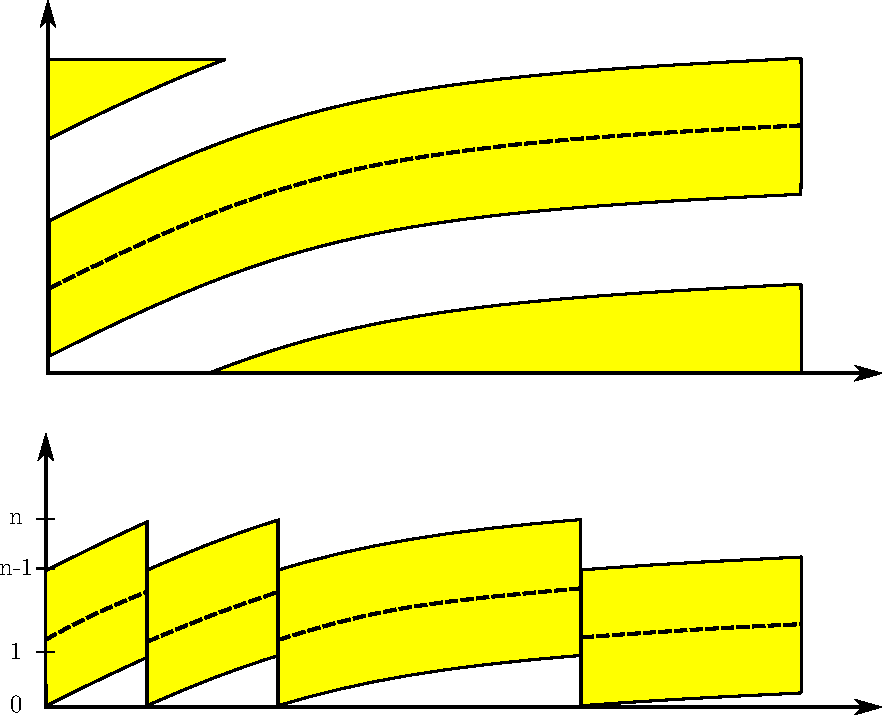
\includegraphics[width=0.45\linewidth]{rectification.pdf}
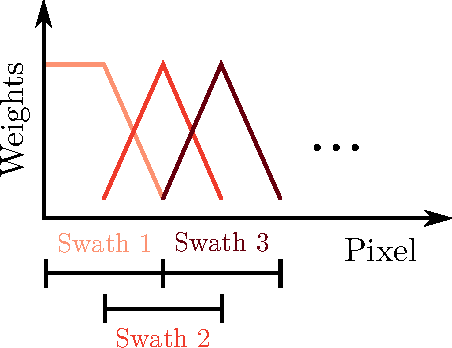
\includegraphics[width=0.45\linewidth]{swath_weights.pdf}
\end{center}
\caption{\it Left: Illustration of swath rectification. Right: The weights for combining the spectra from overlapping swaths.}
\label{fig:swaths}
\end{figure}

\begin{figure}[ht]
    \begin{center}
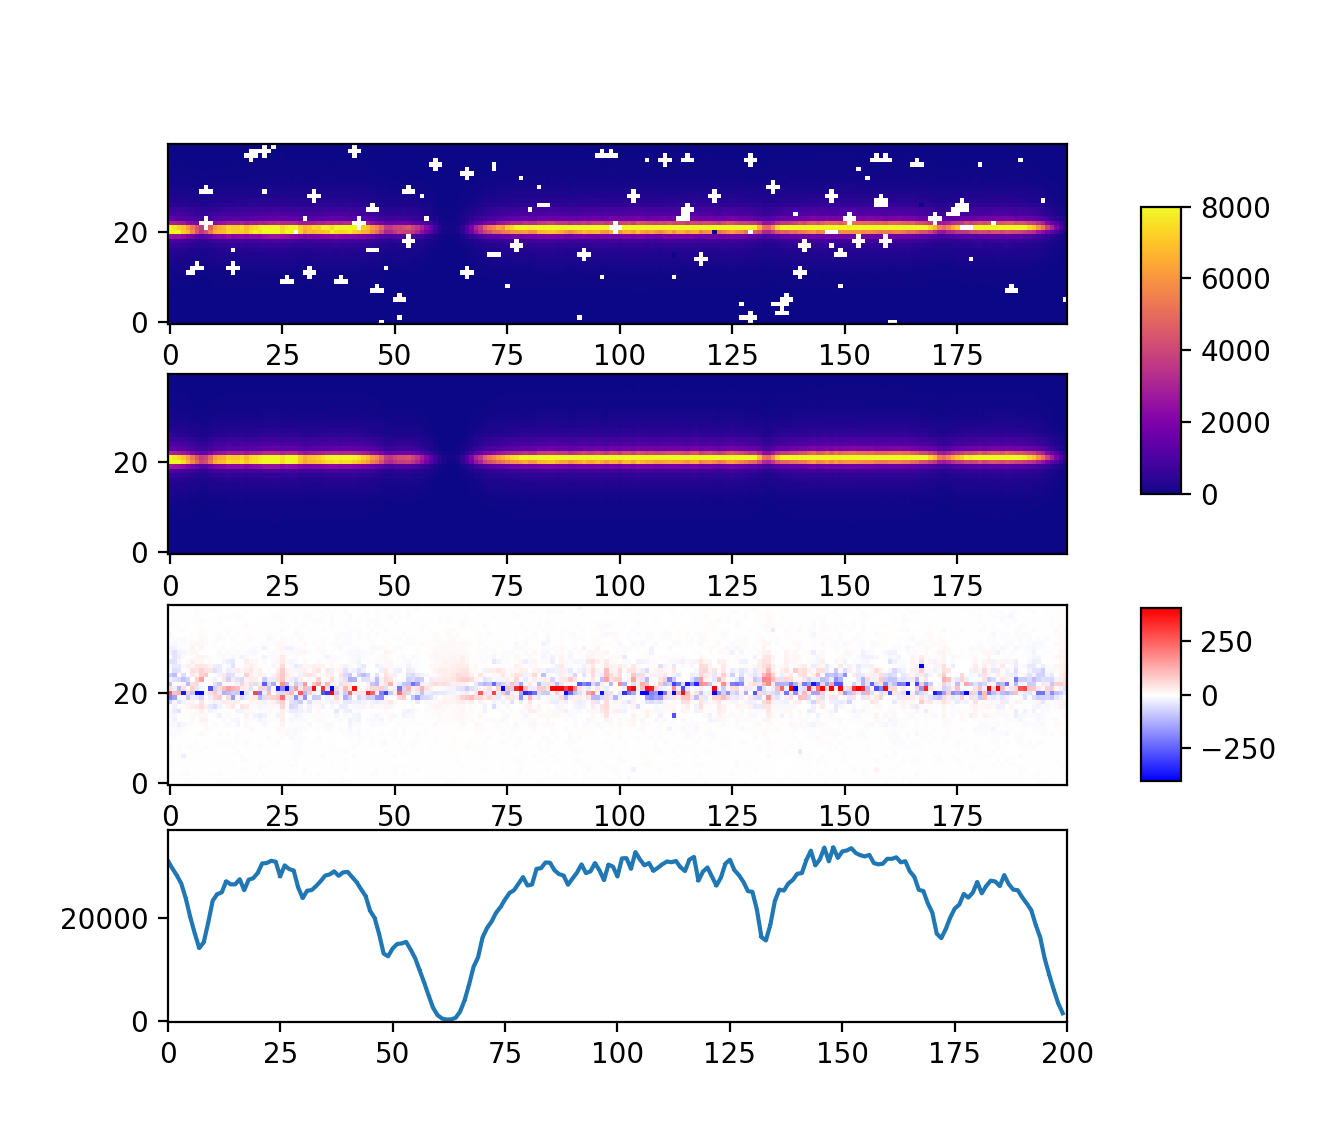
\includegraphics[width=0.85\linewidth]{extr_model.png}
\end{center}
\caption{\it foo}
\label{fig:extrmodel}
\end{figure}

The optimal extraction along the tilted and curved slit is a centerpiece of the
\instrument\ DRS and several recipes make use of it. Full details and
mathematical description can be found in \cite{2021A&A...646A..32P}. Here, we
simply summarize the most important practical implications from a user
perspective.

To extract a spectral order from a calibrated 2D frame into a 1D spectrum, using
a \emph{trace} from the TW table, the following steps are carried out:
\begin{itemize}
    \item Calculate the extraction height from the edge-polynomials, if not
    explicitly given via \texttt{-{}-extract\_height}.
    \item Cut out a rectangular region around the mid-line, called a
    \emph{swath} from the frame, using the height and the value of
    \texttt{-{}-extract\_swath\_width}.
    \item Rectify the swath by shifting columns by integer values such that the
    mid-line only retains values between $0\ldots 1$, like illustrated in
    \figref{fig:swaths} (left).
    \item Iteratively approximate the swath surface by two vectors: the spectrum
    along the mid-line and the slit-function along the slit projection, taking
    its changeing tilt into accont. The slit function is oversampled by a factor
    \texttt{-{}-extract\_oversample}.
    \item Step by a half swath-width to the next one, and repeat. This way
    swaths overlap fully and the order effectively gets extracted twice.
    \item Once all swaths are extracted, the spectra from each are merged into
    one, with linearly in-/decreasing weights, as in \figref{fig:swaths}
    (right).
    \item The spectrum and slit-functions are saved, and used to reconstruct a 2D model of the frame, saved separately.
    \item The errors are estimated from the residual between data and model.
\end{itemize}

A major advantage of this extraction algorithm is that it makes not assumption about the slit-function, except that it does not change within a swath.

In addition, the model by design cannot approximate features that are not present in all pixels that contribute to a certain bin in the spectrum or the slit-function. This makes spectra robust towards e.g.~cosmic rays.

\subsection{Recipes Algorithms} 
\label{sec:algorithms-recipes}


\subsection{Nodding}
\label{sec:nodd}

Nodding sequence \texttt{SEQ.NABCYCLES}
\texttt{SEQ.NODPOS}

first combined, then calibs applied, then subtracted, then extraction

\subsection{Order Tracing}
\label{sec:ordertrace}

smooth in x.
smooth strongly in y and compare to unsmoothed, threshold.
unify clusters.
label them.
threshold minimum number od pix in cluster.
fit polynomial to all pix.
fit edges.

\subsection{Wavelength calibration}

There are several ways to calibrate the wavelength scale, and each corresponds to one of the values that the parameter \texttt{-{}-wl\_method} of \texttt{cr2res\_util\_wave} can take.

With \texttt{-{}-wl\_method=XCORR} the provided catalog of lines gets made into a synthetic spectrum that is cross-correlated with the extracted lamp spectrum. Each detector-order is calibrated separately.

The recipe \texttt{cr2res\_cal\_wave} combines two methods into one recipe,
one for the UNE lamp frames, and the one for the FPET. The result from the former gets passed on to the latter, if both lamp inputs are present. If not, then only the appropriate method is applied.